\documentclass[../PS6_RapportFinal.tex]{subfiles}

\begin{document}
\graphicspath{{img/}{tex/img/}}

\section{Assemblage du corps principal}

Comme expliqué dans la partie \ref{conceptionechangeur}, l'échangeur est constitué de deux tôles de 2 mm d'épaisseur en acier. Celles-ci ont été pliées puis soudées l'une à l'autre, afin de réaliser un corps parallélépipédique. Bien entendu, divers perçages ont été réalisés au préalable : certains (au nombre de 10) pour accueillir les raccords sur la partie inférieure, ainsi que deux autres (latéraux) permettant la fixation du raccord au réseau hydraulique.

\begin{figure}[h]
\begin{center}
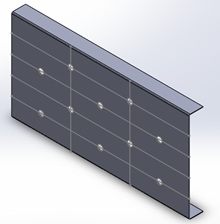
\includegraphics{3_1_capot_inferieur.png}
\caption[width=10cm]{Capot inférieur du corps principal}
\label{tube_aluminium} 
\end{center}
\end{figure}

\begin{figure}[h]
\begin{center}
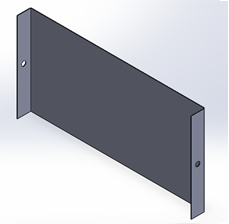
\includegraphics{3_1_capot_superieur.png}
\caption[width=10cm]{Capot supérieur du corps principal}
\label{tube_aluminium} 
\end{center}
\end{figure}


\end{document}